\documentclass[10pt,a4paper]{article}

\usepackage[left=3.5cm, right=3.5cm]{geometry}

\usepackage[utf8]{inputenc}
\usepackage[english]{babel}
\usepackage[english]{isodate}
\usepackage[parfill]{parskip}
\usepackage{hyperref}			%Hyper links and references
\usepackage{graphicx}			%Figures
\usepackage{subcaption}			%Figures side by side
\usepackage{xcolor}				%textcolor
\usepackage{amsmath}			%math environment
\usepackage{enumitem}			%description
\usepackage{listings}			%command line
\usepackage{url}				%paths
\usepackage{cite}				%Citations

%Draw figures
\usepackage{tikz}				
\usetikzlibrary{calc,positioning,shadows.blur,decorations.pathreplacing}


\newcommand*\rfrac[2]{{}^{#1}\!/_{#2}}

\hypersetup{
    colorlinks=true,
    linkcolor=black,
    filecolor=black,      
    urlcolor=blue,
}

\pagenumbering{arabic}


\begin{document}

\title{DUNE Vehicle Simulator (AUVs)}
\maketitle

\tableofcontents
\newpage

\section{Preamble}
The DUNE vehicle simulator provides a way to interact with the core system without a hardware vehicle by simulating it's behaviour using a physical model. The simulator then dispatches IMC messages, corresponding to those of a real vehicle, to the remaining (non-simulated) DUNE tasks. This feature is useful for testing and learning purposes.
 
\par The present document provides a general description of DUNE's simulator and its components, and it is intended to be read alongside the simulator code. For someone with a basic knowledge of the simulator the different sections can be consulted independently. This document is structured as follows:

\begin{itemize}
\item A quick start guide provides an easy and fast way to get the simulator up and running, so the user is able to interact with the system directly.
\item A brief description of the configuration files is given, with special emphasis on the \path{simulator.ini} file.
\item Description of the different vehicle simulator task components, the implemented physical model, and an explanation of the implemented structure.
\item Description of the remaining simulated components, such as sensors and actuators.
\end{itemize}

A coherent nomenclature has been used in task descriptions as follows: \textbf{method/class} names, \textit{IMC message} names, ``variable" names \path{files/paths} and
\begin{lstlisting}[language=bash, frame=single]
  commands.
\end{lstlisting}

\section{Quick Start}
This document assumes the reader has already obtained and built the source code for both DUNE and NEPTUS systems, otherwise a guide to do so can be found \href{https://github.com/LSTS/dune/wiki}{here}.

To run a basic simulation follow these steps:

\begin{enumerate}
\item Start a DUNE instance by running the command:

\begin{lstlisting}[language=bash, frame=single]
  ./dune <configuration file> -p Simulation
\end{lstlisting}

in the DUNE build directory. The configuration file (Section \ref{configuration_file}) determines the vehicle to simulate. Several have already been developed and can be found in the \path{etc} folder. The profile must be set to 
\begin{lstlisting}[language=bash, frame=single]
  Simulation
\end{lstlisting}
in order to enable the appropriate simulation entities,  using the option 
\begin{lstlisting}[language=bash, frame=single]
  -p
\end{lstlisting}
For this example we will be using the \path{lauv-xplore-1.ini} configuration file, so the complete command should be:
\begin{lstlisting}[language=bash, frame=single]
  ./dune lauv-xplore-1.ini -p Simulation
\end{lstlisting}

\item You must start an instance of NEPTUS to control your vehicle. This is done by running the command:
\begin{lstlisting}[language=bash, frame=single]
  ./neptus.sh
\end{lstlisting}
in the NEPTUS home directory. A more detailed reference for NEPTUS can be found \href{https://lsts.pt/neptus/manual/trunk/index.html}{here}. Now, to control your simulated vehicle, you simply have to follow the steps outlined in the \href{https://whale.fe.up.pt/neptus/manual/trunk/commonTasks.html#operating-instructions}{Operating Instructions} section.


\iffalse
\item Next go to ``Console Open/Builder" to open the console interface, then go to "File \textgreater Open Console" and select a console file (ncon) when prompt. In this example we will be using the \textit{lauv.ncon} console, since we are dealing with a \textbf{L}ight \textbf{A}utonomous \textbf{U}nderwater \textbf{V}ehicle.

\item In the center window you should see a map of the mission area, on the right you should see the vehicle operation widgets and a drop down menu for vehicle selection. Select the vehicle corresponding to your configuration file, in our case the \textit{lauv-xplore-1}. If you cannot find your vehicle go to ``Advanced \textgreater Set Main Vehicle..." and select your vehicle when prompt.

\item Next you must define a plan for your vehicle to follow. Click on the ``Plan Edition" icon on the left side and select your vehicle when prompt. Now, by right clicking on the map you wll be able to add a series of maneuvers to your plan. Start by adding a simple "goto maneuver and save your plan, giving it a custom id.

\item Finally select your plan from the plan list on the right and press the ``Send Selection Plan" (upward arrow) to send the plan maneuvers to the simulated vehicle. Then simply press the (green) "Start Plan button to make the simulated vehicle execute the maneuvers. 
\fi
\end{enumerate}

\section{Configuration File}
\label{configuration_file}

\par DUNE works based on a system of modular tasks that can be called and configured using configuration \path{.ini} files. This allows the construction of entire vehicle control systems by simply adding and configuring instances of tasks with no alterations to the code. If a component is added or modified, either hardware (like a sensor or motor) or software (like a controller), the system can be changed through the configuration files, provided the appropriate tasks are already implemented.  

\par In this document we will only give a brief overview of the configuration files used in simulation, aimed at explaining the necessary configuration parameters. The basic workings and features of configuration files can be found on the \href{https://github.com/LSTS/dune/wiki/Additional-configuration-file-features}{Additional configuration file features} section of the DUNE documentation.

\subsection{Vehicle configuration}

\par When we start a DUNE instance the vehicle configuration file sets which tasks will be used (occasionally more than one instance of each task) and their parameters. This contains general vehicle parameters including the vehicle name and several vehicle specific configurations such as maximum allowed depth, speed, battery capacity etc. The file can also include other configuration files, allowing for the separation of the configuration into several files and reuse of general configurations across multiple vehicles. These can call on hardware specific tasks, depending on what is physically implemented, and more generic tasks, such as control and maneuvering algorithms, required by different vehicles. In the case of AUVs it calls on the \path{auv/basic.ini} file, which contains configurations that are required by all AUVs. The main file can also include parameter overrides for task instances initialized in other files, if we wish to change these particular parameters for our vehicle setup.

\subsection{Basic configuration}

\par The basic configuration file does not call on any task instances per se, instead it acts as a compilation of other configuration files that implement different generic instances required for operation of all vehicle of that type. In the case of AUVs this includes:

\begin{itemize}
\item plans
\item transports
\item simulator
\item control
\item navigation
\item maneuvers
\item monitors
\item supervisors
\item general
\end{itemize}

In this document we are interested in the \path{simulator.ini} configuration file.

\subsection{Simulator configuration}

The \path{simulator.ini} is the main configuration file for the simulator. This calls on all DUNE task instances necessary for the simulation engine, including:

\begin{itemize}

%VSIM
\item \href{https://www.lsts.pt/docs/dune/dune-2017.01.0-dmsmw/d2/d2f/structSimulators_1_1VSIM_1_1Task.html}{VSIM} - \href{https://www.lsts.pt/docs/dune/dune-2017.01.0-dmsmw/d3/d5d/structSimulators_1_1VSIM_1_1Arguments.html}{Arguments}

%GPS
\item \href{https://www.lsts.pt/docs/dune/dune-2017.01.0-dmsmw/db/da2/structSimulators_1_1GPS_1_1Task.html}{GPS} - \href{https://www.lsts.pt/docs/dune/dune-2017.01.0-dmsmw/d1/dd3/structSimulators_1_1GPS_1_1Arguments.html}{Arguments}

%LBL
\item \href{https://www.lsts.pt/docs/dune/dune-2017.01.0-dmsmw/d0/dd2/structSimulators_1_1LBL_1_1Task.html}{LBL} - \href{https://www.lsts.pt/docs/dune/dune-2017.01.0-dmsmw/d4/dde/structSimulators_1_1LBL_1_1Arguments.html}{Arguments}

%Environment
\item \href{https://www.lsts.pt/docs/dune/dune-2017.01.0-dmsmw/db/d16/structSimulators_1_1Environment_1_1Task.html}{Environment} - \href{https://www.lsts.pt/docs/dune/dune-2017.01.0-dmsmw/d1/d85/structSimulators_1_1Environment_1_1Arguments.html}{Arguments}

%Leaks
\item \href{https://www.lsts.pt/docs/dune/dune-2017.01.0-dmsmw/d2/d45/structSimulators_1_1Leaks_1_1Task.html}{Leaks} - \href{https://www.lsts.pt/docs/dune/dune-2017.01.0-dmsmw/dd/d5d/structSimulators_1_1Leaks_1_1Arguments.html}{Arguments}

%Motor
\item \href{https://www.lsts.pt/docs/dune/dune-2017.01.0-dmsmw/d1/d8f/structSimulators_1_1Motor_1_1Task.html}{Motor} - \href{https://www.lsts.pt/docs/dune/dune-2017.01.0-dmsmw/d9/dd8/structSimulators_1_1Motor_1_1Arguments.html}{Arguments}

%Servos
\item \href{https://www.lsts.pt/docs/dune/dune-2017.01.0-dmsmw/df/d90/structSimulators_1_1Servos_1_1Task.html}{Servos} - \href{https://www.lsts.pt/docs/dune/dune-2017.01.0-dmsmw/d3/dcd/structSimulators_1_1Servos_1_1Arguments.html}{Arguments}

%Gaussian
\item \href{https://www.lsts.pt/docs/dune/dune-2017.01.0-dmsmw/d9/d36/structSimulators_1_1Gaussian_1_1Task.html}{Gaussian} - \href{https://www.lsts.pt/docs/dune/dune-2017.01.0-dmsmw/d6/d7b/structSimulators_1_1Gaussian_1_1Arguments.html}{Arguments}
\end{itemize}

and defines values for each of its necessary arguments. An explanation of all task specific parameters would be too cumbersome, therefore we refer the reader to the arguments documentation in the list above. However we mention some general parameters:
The ``Enabled" flag is common to all instances and indicates under which profile the task should run: 
\begin{description}
\item[Always] - always called
\item[Never] - never called
\item[Hardware] - called when the physical hardware is detected
\item[Simulation] - runs the simulator tasks
\end{description}
The ``Execution Frequency" determines the frequency at which the periodic tasks should run (in Hz). The ``Entity Label" simply attributes a name to the entity. 


\subsection{vsim-models.ini}
\label{vsim_models_ini}

\par \path{simulator.ini} also includes the \path{vsim-models.ini} configuration file, which defines the parameters necessary for the simulation of vehicle physics. For the case of AUVs these include:

\begin{description}[leftmargin=19em,style=nextline] %{Quadratic Drag Coefficients}

\item[Gravity] The gravity acceleration in the $\left\{x, y, z\right\}$ components, in $m/s^2$.

\item[Type] The vehicle type: UUV, ROV, ASV.

\item[Mass] The vehicle mass in $Kg$.

\item[Buoyancy] The buoyancy force in the $\left\{x, y, z\right\}$ components, in $N$.

\item[Volume] The vehicle's dimensions in the $\left\{x, y, z\right\}$ components, in $m$.

\item[Inertial Matrix] The diagonal coefficients of the vehicle's inertia tensor in 6 DOF, with component order: $\left\{ c_{1,1}, c_{2,2}, c_{3,3}, c_{4,4}, c_{5,5}, c_{6,6} \right\}$. Values for these coefficients were taken from \cite{braga}.

\item[Linear Drag Coefficients] Damping matrix linear coefficients, with component order:
$\left\{ c_{1,1}, c_{2,2}, c_{3,3}, c_{4,4}, c_{5,5}, c_{6,6}, c_{2,6}, c_{3,5}, c_{5,3}, c_{6,2} \right\}$. Values for these coefficients were taken from \cite{braga}.

\item[Quadratic Drag Coefficients] Damping matrix quadratic coefficients, with component order:
$\left\{ c_{1,1}, c_{2,2}, c_{3,3}, c_{4,4}, c_{5,5}, c_{6,6}, c_{2,6}, c_{3,5}, c_{5,3}, c_{6,2} \right\}$. Values for these coefficients were taken from \cite{braga}.

\item[Added Mass Coefficients] The diagonal coefficients of the vehicle's added mass matrix, with component order: $\left\{ c_{1,1}, c_{2,2}, c_{3,3}, c_{4,4}, c_{5,5}, c_{6,6} \right\}$. \textcolor{red}{Onde estao os valores? Nao esta junto com a matrix inercial??}

\item[Body Lift Coefficients] Lift matrix coefficients, with component order: $\left\{ c_{2,2}, c_{2,6}, c_{3,3}, c_{3,5}, c_{5,3}, c_{5,5}, c_{6,2}, c_{6,6}\right\}$. Values for these coefficients were taken from \cite{braga}.

\item[Fin Count] The number of fins in the vehicle.

\item[Fin Force \#]	The maximum force fin \# is able to produce, in the $\left\{x, y, z\right\}$ components, in $N$.

\item[Fin Position \#] The position of fin \# in $\left\{x, y, z\right\}$, in $m$.

\item[Engine Count] The number of engines in the vehicle.

\item[Engine Parameters \#] Parameters of engine \# with order: $\left\{b_1, b_2, RPM_{max}\right\}$. Where $\left(b_1, b_2\right)$ are the coeficients found in equation (4.7) of \cite{fossen} and $RPM_{max}$ is the maximum engine's rpm.

\item[Engine Position \#] The position of engine \# in $\left\{x, y, z\right\}$, in $m$.

\item[Engine Orientation \#] The orientation of engine \# as $\left\{\psi, \theta\right\}$ angles, in $rad$.

\item[Engine Max Force] The maximum force engine \# is able to produce, in $N$.

\end{description}

Notice a body fixed reference frame is used, centered at the vehicle's CG, with x pointing forward along the longitudinal axis of the vehicle, y pointing right along the lateral axis of the vehicle, and z pointing down along the vertical axis of the vehicle. $\phi$, $\theta$, and $\psi$, are the Euler angles that define the body reference frame rotation relative to the fixed reference frame (usually Earth) in the 3-2-1 order: $Earth \rightarrow \psi \rightarrow \theta \rightarrow \phi \rightarrow body$.

\section{Simulator}
\par DUNE has the capability to simulate different types of systems. It can simulate the behaviour of AUVs, UAVs (fixed-wings), ROVs and ASVs. Once DUNE is running a simulated system, NEPTUS will interact with it as it would with a real system running DUNE.

\par The DUNE simulator can be separated in 2 components: the ``dynamics component", the main simulation engine implemented in the Vehicle SIMulator task, and the ``sensor components". 

\par The ``dynamics component" comprises the physical model that describes vehicle movement, and is implemented in the VSIM task. This model can be found in \cite{braga}, which is a simplification of the more complete model found in \cite{fossen}. Here we include the rigid body dynamics, given by the inertia tensor, and the hydrodynamic forces applied to the vehicle, which include: the added mass force, due to the surrounding fluid the vehicle has to displace; the damping force, caused by skin friction and vortex shedding; and the restoring forces, where we include buoyancy and gravity. Furthermore the vehicle is assumed to have a prolate ellipsoid shape, which determines the calculation of coefficients for the aforementioned forces. The vehicle state (position, attitude and velocity) is then obtained by integrating the accelerations, obtained from the hydrodynamic forces, using a simple Euler algorithm.

\par The "sensor components" correspond to the simulation of everything else from sensor information to mechanical components such as motors and other actuators.

\par Bellow we give a more detailed description of the VSIM task, which is subdivided into several modular components, and the remaining simulated entities. A schematic diagram of the simulator entities can be found in figure \ref{simulator_overview_diagram}, and we advise the reader to keep this diagram in mind throughout the document.

\begin{figure}[h]
  \centering
  	\includegraphics[width=1.0\textwidth]{figures/Overview_diagram.png}
  \caption{Simulator overview diagram.}
  \label{simulator_overview_diagram}
\end{figure}


\section{VSIM Task \href{https://www.lsts.pt/docs/dune/dune-2017.01.0-dmsmw/d2/d2f/structSimulators_1_1VSIM_1_1Task.html}{\textsuperscript{*}}}

The Vehicle SIMulator acts as the main task in DUNE's simulator engine. It is responsible for creating a virtual environment which contains the physical properties required in simulation, coordinating IMC messages from other entities and constructing and advancing the vehicle's simulated state.

\par When the task is started the configuration parameters are assigned in the constructor. The \textbf{onResourceInitialization} method initializes the simulated world by generating a World and Vehicle instances containing gravity acceleration and vehicle dynamical properties, such as mass, buoyancy, inertial matrix, etc (Subsections \ref{world_class} and \ref{vehicle_class}). The Vehicle pointer is then passed to the World object and a time step is defined for numerical integration purposes, completing the virtual world setup.

\par The task consumes an initial \textit{GpsFix} message, from the simulated GPS, containing the vehicles reference origin. If the message is of the manual input type the method sets the vehicle's offset $\left(x,y,z\right)$ positions to 0 and orientation to the course over ground provided by the message. The method also sets the vehicle's reference origin (lat, lon, height). These parameters are then assigned to the ``m\_sstate" \textit{SimulatedState} message (analogous to the \textit{EstimatedState} message used for real vehicles).

\par The dead reckoning navigation where we separate a reference origin, in WGS84 coordinates, and offset position, in $m$, greatly facilitates calculations since we are free to define the origin of our referential. Obtaining the actual vehicle position on the Earth's reference frame is then a simple matter of adding the offsets to the reference origin with the appropriate coordinate conversion. Finally the method saves the start time for use in later calculations and activates the task.

\par The periodic task then calls on the \textbf{takeStep} method, from the World object, to advance the vehicle's position, attitude, linear and angular velocities by the previously defined time step. The ``m\_sstate" message is then updated with the new state, by also taking into account the water current speeds obtained in the constructor, and the message is dispatched.

\par The task also consumes a \textit{ServoPosition} and \textit{SetThrusterActuation} messages to set the vehicles fin positions and engine thrust, respectively. These values are later used to compute forces applied to the vehicle (Subsections \ref{engine_class} and \ref{fin_class}).


\subsection{Factory Class \href{https://www.lsts.pt/docs/dune/dune-2017.01.0-dmsmw/db/d0e/classSimulators_1_1VSIM_1_1Factory.html}{\textsuperscript{*}}}
\label{factory_class}

\par The factory class has two methods: \textbf{produceWorld} and \textbf{produceVehicle}, which return pointers to World and Vehicle objects, respectively. These objects are constructed using the configuration parameters found in \path{vsim_models_ini} (Subsection \ref{vsim_models_ini}). They are called once, on the \textbf{onResourceInitialization} method of the VSIM task, to produce the virtual environment.

\subsection{World Class \href{https://www.lsts.pt/docs/dune/dune-2017.01.0-dmsmw/d9/d88/classSimulators_1_1VSIM_1_1World.html}{\textsuperscript{*}}}
\label{world_class}

\par The World class represents the simulated world and it is from here we can call the methods that advance the vehicle state. A World object holds values for gravity acceleration components and a list of Object and Vehicle pointers, which can be added to it via the \textbf{addObject} and \textbf{addVehicle} methods.

\par The state of the Objects and Vehicles in the World object is advanced by calling the \textbf{takeStep} method. Here the \textbf{applyForces} method triggers the calculation of the forces applied to all Objects and Vehicles saved in World. Then, the \textbf{update} method, triggers the calculation of the new state of the Objects and Vehicles based on the forces applied to them. 

\subsection{Object Class \href{https://www.lsts.pt/docs/dune/dune-2017.01.0-dmsmw/d3/dd8/classSimulators_1_1VSIM_1_1Object.html}{\textsuperscript{*}}}
\label{object_class}

\par The Object class represents a generic simulated object. An Object object holds the properties of a physical object, such as mass, inertia matrix, linear and quadratic drag coefficients. These parameters can be set using the \textbf{setMassProp}, \textbf{setLinearDragCoef}, \textbf{setQuadraticDragCoef} methods. It also holds the object state, meaning position, orientation, linear and angular velocity. Values for the initial position and orientation can be set using the \textbf{setPosition} and \textbf{setOrientation} methods.

\par The \textbf{applyForces} method in the Object class triggers the calculation of all forces applied to the object and adds them to a force array ``m\_forces". This is a six element array that holds the total force and torque applied to the object in each of the six components ($\left\{x,y,z,\phi, \theta,\psi\right\}$). In the case of a simple object (meaning no inherited classes) only the \textbf{applyDragForces} method is called. Here the drag forces applied to the object are calculated based on the object's state, using the formula: $F_{Drag} = D_{linear} \cdot \vec{\nu} + D_{quad}\left(\vec{\nu}\right) \cdot \vec{\nu}$, where $D_{linear}$ is the linear drag matrix, $D_{quad}\left(\vec{\nu}\right)$ is the quadratic drag matrix and $\vec{\nu} = \left\{u,v,w,p,q,r\right\}$ is the linear and angular velocity vector \cite{braga}.

\par The \textbf{update} method then uses these calculated forces to advance the object's state. The method starts by calculating the total acceleration in each component: $\dot{\nu}_{n} = \frac{F_{n}}{I_{n}}$, where $F_{n}$ is the force along the component $n = \left\{x, y, z, \phi, \theta, \psi\right\}$ (obtained from ``m\_forces") and $I_{n}$ is the respective inertial matrix coefficient. Then the velocity in the earth fixed reference frame is obtained using the formulas $\dot{\eta}_1=J_{1}\left(\eta_2\right) \cdot \nu_1$ and $\dot{\eta}_2=J_{2}\left(\eta_2\right) \cdot \nu_2$, where $\dot{\eta}_1$ and $\dot{\eta}_2$ are the linear and angular velocities in the earth fixed frame, $\nu_1$ and $\nu_2$ are the velocities in the body fixed frame and $J_{1}\left(\eta_2\right)$ and $J_{1}\left(\eta_2\right)$ are the rotation matrices described in \cite{fossen}. The new positions and velocities are then calculated: $\eta_{t+1} = \eta_{t} + \dot{\eta_{t}} \cdot \Delta t$ and $\nu_{t+1} = \nu_{t} + \dot{\nu_{t}} \cdot \Delta t$ respectively, where $\Delta t$ is a previously defined time step. The ``m\_forces" array is then reset to 0 so it can be used in the next iteration.

\subsection{Vehicle Class \href{https://www.lsts.pt/docs/dune/dune-2017.01.0-dmsmw/d4/d43/classSimulators_1_1VSIM_1_1Vehicle.html}{\textsuperscript{*}}}
\label{vehicle_class}

\par The Vehicle class represents a generic simulated vehicle. This class inherits from the Object class and expands upon its methods, more specifically, by adding control forces (internal forces used to control the vehicle) such as the force produced by an engine, as discussed in Subsection \ref{engine_class}. More control forces, such as fins, can be implemented in more specific vehicle subclasses, such as the UUV class, as we will see in Subsection \ref{uuv_class}). 

\par The parameters for these control forces are obtain by the Factory, from \path{vsim-models.ini}, and stored in a Force (Subsection \ref{force_class}) pointers list: ``m\_vehicle\_forces" using the \textbf{addForce} and \textbf{addEngine} methods. The engine actuation can be set via the \textbf{updateEngine} method, called in VSIM, which receives the engine id and desired actuation, then triggers the \textbf{updateact} method, which searches the ``m\_vehicle\_forces" for the specified id and sets the desired actuation when found.

\par When the \textbf{applyForces} method of a Vehicle object is called, it triggers not only the \textbf{applyDragForces} but also the subclass method \textbf{applyControlForces}. This method triggers the calculation of all Forces in ``m\_vehicle\_forces" and adds their respective values to ``m\_forces". This is later used in the calculations to advance the Vehicle state as we saw at the end of Subsection \ref{object_class}.

\subsection{UUV Class \href{https://www.lsts.pt/docs/dune/dune-2017.01.0-dmsmw/d1/d3b/classSimulators_1_1VSIM_1_1UUV.html}{\textsuperscript{*}}}
\label{uuv_class}

\par The UUV class represents a simulated \textbf{U}nmanned \textbf{U}nderwater simulated \textbf{V}ehicle. This class inherits from the Vehicle class and expands upon it by adding more physical characteristics, such as the volume, center of buoyancy, added mass and body lift coefficients. It also adds an extra control force provided by the Fins' objects.

\par These parameters and control forces are obtain by the Factory from \path{vsim-models.ini} and added to the vehicle, using the constructor, \textbf{setBuoyancyPosition}, \textbf{setAddedMassCoef} and \textbf{setBodyLiftCoef} methods. The fin actuation can be set via the \textbf{updateFin} method, called in VSIM, which receives the fin id and desired actuation (for fins the actuation corresponds to the fin angle in radians) then triggers the \textbf{updateact} method, which searches the ``m\_vehicle\_forces" for the specified id and sets the desired actuation when found.

\par When the \textbf{applyForces} method of a UUV object is called it triggers the \textbf{applyDragForces} and \textbf{applyControlForces} methods, from the Vehicle class, plus the \textbf{applyCoriolisForce} and \textbf{applyRestoringForcesMoments} from the UUV class.

\par The \textbf{applyCoriolisForce} method calculates the Coriolis and lift forces applied to the vehicle and adds them to ``m\_forces". The Coriolis force is calculated based on the vehicle's state, using the formula: $F_{Coriolis} = C\left(\vec{\nu}\right) \vec{\nu}$, where $C\left(\vec{\nu}\right)$ is the Coriolis matrix and  $\vec{\nu}$ is the velocity vector. The lift force is calculated using: $F_{lift} = L\left(\vec{\nu}\right) \vec{\nu} \left(\vec{\nu}\cdot \vec{e_x}\right)$, where $L\left(\vec{\nu}\right)$ is the Lift matrix and  $\vec{\nu}\cdot \vec{e_x} = u$ is the linear velocity in the $x$ component \cite{braga}.

\par The \textbf{applyRestoringForcesMoments} method calculates the gravity and buoyancy forces applied to the vehicle. The gravitational force is calculated using: $F_{g} = m\cdot g$, where $m$ is the vehicle mass and $g$ is the gravity acceleration. The buoyancy force is calculated using: $F_{b}=g\cdot \rho \cdot V_{sub}$, where $\rho$ is the water density and $V_{sub}$ is the submerged volume of the vehicle. Note the force application points are different, since the center of buoyancy is set to be slightly above the center of gravity, to ensure roll stability. The force components are then added to ``m\_forces".

\subsection{Force Class \href{https://www.lsts.pt/docs/dune/dune-2017.01.0-dmsmw/d0/d49/classSimulators_1_1VSIM_1_1Force.html}{\textsuperscript{*}}}
\label{force_class}

\par The Force class represents a generic force applied to the object or vehicle and is the base class for the Engine and Fin subclasses. The class holds the force application position and the maximum possible force values in the $\left\{x,y,z\right\}$ components, set using the \textbf{setPosition} and \textbf{setForce} methods. The class also holds some force properties such as if the force, and its application position, are in the inertial referential and if it is a linear force or a torque. The actual calculations and implementation are in the Engine and Fin subclasses.

\subsection{Engine Class \href{https://www.lsts.pt/docs/dune/dune-2017.01.0-dmsmw/d3/df7/classSimulators_1_1VSIM_1_1Engine.html}{\textsuperscript{*}}}
\label{engine_class}

\par The Engine class represents the force produced by a propeller in a simulated vehicle. This class inherits from the Force class, expanding upon it to add the characteristics of an engine produced force. 

\par The \textbf{setEngine} method sets the position and maximum force arrays, from the Force class, plus the engine's orientation, an identifying id and the total maximum force produced by the engine. Note however that in this particular case the maximum force array does not contain the maximum force in each component, instead the components are $\left\{b_1, b_2, RPM_{max}\right\}$, where $b_1$ and $b_2$ are parameters used to calculate the thrust force from the rpm values and $RPM_{max}$ is the maximum engine's rpm, used to calculate the rpm from the received actuation value.

\par The desired engine actuation is set using the \textbf{updateAct} method, called in the \textit{SetThrusterActuation} consume method in VSIM. This value represents a relative magnitude in the range $\left[-1,1\right]$.

\par When the \textbf{applyForce} method is called it triggers the \textbf{getEngineProducedForce} method which calculates the engine forces and adds them to ``m\_forces". The method starts by obtaining the engine's rps from the actuation: $rps = act\cdot \frac{RPM_{max}}{60}$. The rps is then used to calculate the propellers total thrust force by using the formula: $F_{thrust} = \left(b_1 rps - b_2 \left|\vec{\nu}\right| \right) \cdot \left| rps \right|$, (equation (4.7) from \cite{fossen}). The force is then projected to its 6 different components and returned.

\subsection{Fin Class \href{https://www.lsts.pt/docs/dune/dune-2017.01.0-dmsmw/d0/dfa/classSimulators_1_1VSIM_1_1Fin.html}{\textsuperscript{*}}}
\label{fin_class}

\par The Fin class represents the force produced by a fin in a simulated vehicle. This class inherits from the Force class, expanding upon it athe characteristics of an engine produced force. 

\par The \textbf{setFin} method is used to set the position and maximum force arrays, from the Force class, plus a local identifying id.

\par The desired fin actuation is set using the \textbf{updateAct} method, called in the \textit{ServoPosition} consume method in VSIM. This value represents the fin angle in radians, the relative actuation magnitude used in the calculations can then be obtained by using: $act = \frac{\alpha}{\alpha_{max}}$, where $\alpha$ is the fin angle in $rad$ and $\alpha_{max}$ is the fin's maximum angle in $rad$.

\par When the \textbf{applyForce} method is called, in the Vehicle class, it triggers the \textbf{getFinProducedForce} and \textbf{getFinProducedTorque} methods which calculate the fin's forces and adds them to ``m\_forces".

\par The \textbf{getFinProducedForce} method starts by checking if $act$ is within the $\left[-1,1\right]$ range. Then it calculates the linear forces by using the formula: $\vec{F}_{linear} = \left|\vec{\nu}\right|^2 \vec{F}_{max}\cdot\frac{act}{2}$, where $\vec{F}_{linear}$ is the vector of linear forces and $\vec{F}_{max}$ is the vector of the maximum fin force. The \textbf{getFinProducedTorque} method then calculates the torques by using the formula: $\vec{T} = \vec{r} \times \vec{F}_{linear}$, where $\vec{T}$ is the torque vector and $\vec{r}$ is the fin position vector.

\section{Motor Task \href{https://www.lsts.pt/docs/dune/dune-2017.01.0-dmsmw/d1/d8f/structSimulators_1_1Motor_1_1Task.html}{\textsuperscript{*}}}
\label{motor_task}

\par The simulator's Motor task is responsible for simulating a hardware motor by receiving a \textit{SetThrusterActuation} message, converting the actuation to rotations per minute and dispatching a corresponding \textit{Rpm} message. 

\par This task, however, does not interact directly with VSIM. Instead a \textit{DesiredSpeed} message is received by the \path{Control.AUV.Speed} task which then sends a \textit{SetThrusterActuation} message received by the VSIM and Motor tasks. This is somewhat counterintuitive, however the reason is that the Engine force is calculated using the actuation magnitude and not RPMs. Since these values can be converted interchangeably it becomes easier to use actuation directly, hence the direct message from the control layer. The \textit{SetThrusterActuation} message is nonetheless received by the Motor task, which converts it into a rpm and sends a corresponding \textit{RPM} message back to the Control.AUV.Speed task. This simulates the feedback loop between motor and controller required for thrust corrections. However, in this particular case, it is assumed the rpms are controlled by the simulated hardware and no corrections are made.

\par When the Motor (or any) task is started the configuration parameters from the \path{.ini} file are assigned in the constructor. The \textbf{onResourceInitialization} method initializes the \textit{Rpm} message, which represents the virtual motor's rpms. Some auxiliary variables are also initialized, including a \textbf{MovingAverage} object used to filter rpm values.

\par The task consumes the \textit{SetThrusterActuation} message sent by the control layer and converts the actuation magnitude (in the range $\left[-1, 1\right]$) to an rpm value. The conversion is done using the formula: $rpm =  a\left(\frac{act}{\left| act \right|}\right) + b \cdot act$, where the $a$ and $b$ coefficients where estimated by least squares method using mission data. This rpm value is then saved into an auxiliary variable ``m\_rpm\_new".

\par The periodic task continuously adds ``m\_rpm\_new" to the moving average and sets the current rpm value to the \textit{Rpm} message, then checks the value for a lower threshold and dispatches the message. The message is then received by the control layer which responds with a \textit{SetThrusterActuation} message, simulating the control loop, as seen in figure \ref{simulator_overview_diagram}.

\section{Servos Task \href{https://www.lsts.pt/docs/dune/dune-2017.01.0-dmsmw/df/d90/structSimulators_1_1Servos_1_1Task.html}{\textsuperscript{*}}}
\label{servos_task}

\par The simulator's Servo task is responsible for simulating the vehicle's servo motors by receiving \textit{SetServoPosition} messages, simulating the servos rotation and dispatching a corresponding \textit{ServoPosition} message, in the same way the hardware servos would.

\par When the configuration parameters are assigned in the constructor, or changed, the \textbf{onUpdateParameters} method is triggered. In this case, converts all angular quantities from degrees to radians. The \textbf{onResourceInitialization} method initializes the \textit{ServoPosition} message array, ``m\_positions", which represents the positions of the multiple virtual servos. Each message has an ``id" field to identify servo and a ``value" field with the position of the servo in radians.

\par The task consumes a \textit{SetServoPosition} message from the control layer and sets the servo position based on the received ``id" and ``value" fields. The value is trimmed before assignment to ensure it falls within the $\left[-\alpha_{max}, \alpha_{max}\right]$ range, where $\alpha_{max}$ is the maximum angle attainable by the servo.

\par Depending on the ``limit\_rate" flag the position can be set instantly or iteratively. When the change is instant the \textit{ServoPosition} message is assigned field values and dispatched. Otherwise the desired value is saved on a \textit{SetServoPosition} message array, ``m\_commands". When the task
consumes a \textit{SimulatedState} message, the method computes the maximum rotation allowed in this iteration, using: $rotation_{max} = \Delta t \cdot rate_{max}$, where the $\Delta t$ is the time since the last iteration and $rate_{max}$ is the maximum allowed rotation rate in $rad/s$. The angle change is calculated using: $\Delta \alpha = \alpha_{c} - \alpha_t$, where $\alpha_{c}$ is the desired angle, saved in ``m\_commands", and $\alpha_t$ is the current angle. The value is added to the current position ($\alpha_{t+1} = \alpha_t + \Delta \alpha$) and a message is dispatched. This process repeats until the desired position is reached or a new \textit{SetServoPosition} message is received.

\par The task is also capable of simulating faults, depending on the ``generate\_faults" flag. If active a fault is generated after a configurable time interval and prevents the servo from changing position for a specified period of time.

\section{GPS Task \href{https://www.lsts.pt/docs/dune/dune-2017.01.0-dmsmw/db/da2/structSimulators_1_1GPS_1_1Task.html}{\textsuperscript{*}}}
\label{gps_task}

\par The simulator's GPS task is responsible for simulating a GPS device by sending a \textit{GpsFix} message in the same way a hardware GPS would. The task can also report the ground velocity and the heading (yaw) via \textit{GroundVelocity} and \textit{EulerAngles} messages.

\par The \textbf{onUpdateParameters} method creates a \textit{GpsFix} message with the vehicles reference origin position (latitude, longitude, height), in WGS84 coordinates, and dispatched in the \textbf{onResourceInitialization} method.

\par The periodic task then sends a periodic fix message based on the \textit{SimulatedState} it receives from VSIM. The fix validity, satellites, hdop and hacc fields are assigned the configuration parameters, The total speed over ground is calculated from the received velocity components $sog = \sqrt{u^2 + v^2}$ and the course over ground is assigned the yaw, $cog = \psi$. The position (``lat", ``lon", ``height") is obtained by displacing the received offset coordinates $\left(x,y,z\right)$ in relation to the GPS reference origin. A time stamp is also assigned and the message is dispatched.

\par The task is also capable of sending the speed over ground and course over ground as \textit{GroundVelocity} and \textit{EulerAngle} messages respectively, depending on the ``report\_gv" and ``report\_yaw" flag activation.

\par The task can also consume a \textit{GpsFix} message, originating from a different entity, to update the reference origin position, provided the message is of the manual input type.

\section{LBL Task \href{https://www.lsts.pt/docs/dune/dune-2017.01.0-dmsmw/d0/dd2/structSimulators_1_1LBL_1_1Task.html}{\textsuperscript{*}}}

\par The simulator's LBL task is responsible for simulating a long baseline acoustic positioning system by sending periodic pings (\textit{LblRange} messages) containing the distance between the vehicle and LBL transponders (beacons). Multiple transponders can be configured via a \textit{LblConfig} message.

\par The task is deactivated by default and in order to activate it a \textit{SetEntityParameters} message must be sent. This can be done from the NEPTUS console \href{https://whale.fe.up.pt/neptus/manual/trunk/elements.html#systems-configuration}{System Configuration} tab.

\par The task consumes a \textit{LblConfig} message, which may request one of two operations: set configuration or get configuration. The set configuration message provides information on the virtual beacons, such as position and delay,  needed for calculations. If a get configuration message is received the method responds with a \textit{LblConfig} message containing the beacons configurations.

\par The task also consumes a \textit{GpsFix} message, of the manual input type, which is simply used to check if a fix was obtained (without looking at any of its content). A \textit{SimulatedState} message is also consumed, and saved, for later use in the calculation of the vehicle's distance from the beacons.

\par The main task runs on a loop which checks if the entity is active and ready. This is done by calling the \textbf{ready} method with returns TRUE if a gps fix and lbl configurations were obtained and if the number of beacons is non zero. If so the task will send \textit{LblRange} messages periodically, from each of the beacons, containing its distance from the vehicle. A MessageList iterator is used to keep track of which beacon is being addressed and a Counter object keeps the time between pings. When the Counter overflows the addressed beacon's name is passed to the \textbf{range} method, which calculates the distance between beacon and vehicle and sends the \textit{LblRange} message.

\par The \textbf{range} method receives a beacon name and calculates the distance between vehicle and beacon. The method first searches the \textit{LblConfig} message for the configurations of the specified beacon. If a match is found the distance between vehicles position, from \textit{SimulatedState}, and beacon position, from \textit{LblConfig}, is calculated using the \textbf{WGS84::distance} method. A random value is then added to simulate measurement error. There is also a configurable probability of having a very large error, specified locally in ``c\_huge\_error". Finally a \textit{LblRange} message is dispatched with the range value, simulating the return pings from the LBL transponders.

\par \textcolor{red}{Ver melhor a \textit{LblConfig} message. \textit{UamTxFrame} ??????}


\section{Environment Task \href{https://www.lsts.pt/docs/dune/dune-2017.01.0-dmsmw/db/d16/structSimulators_1_1Environment_1_1Task.html}{\textsuperscript{*}}}

\par The simulator's Environment task is responsible for simulating the forward and bottom distance sensors, by sending \textit{Distance} messages in the same way the hardware sensors would. The task uses collected bathymetry data to simulate ocean depth in a given area and performs calculations for simulated forward and bottom distances based on the vehicle's position. For the forward distance the task is able to simulate a pier, as a strait line obstacle, by defining two coordinate points, $a$ and $b$. The task is also capable of simulating pencil beam scanning, implemented in a local \textbf{PencilBeam} class.

\par The \textbf{onUpdateParameters} method converts all angular quantities from degrees to radians. The \textbf{onResourceAcquisition} method initializes a Random::Generator object, later used to simulate measurement error, and a PencilBeam object, later used to simulate sensor lateral angle.

\par The \textbf{onResourceInitialization} method is where most of the task's setup is performed. It first parses bathymetry data from a configurable file, currently only one is available in \path{etc/simulation/bathymetry-apdl.ini}. The file contains a reference origin latitude and longitude, in WGS84 coordinates, and a series of data points in the form ``$x\ y\ d$" where $x$ and $y$ are the offsets from the origin, in $m$, and $d$ is the distance from water surface to ocean floor.

The data points are used to create a Bounds object, which defines a rectangular region with the $\left(x,y\right)$ data limits, as seen in figure \ref{boundary_limits}.

\begin{figure}[h]
  \centering
  	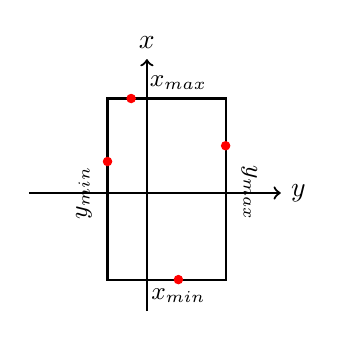
\begin{tikzpicture}

%Axis
\draw[thick,->] (-1.5,0) -- (1.7,0) node[right] {$y$};
\draw[thick,->] (0,-1.5) -- (0,1.7) node[above] {$x$};
%\draw[step=.2cm, gray, very thin] (-1.5,-1.5) grid (1.5,1.5);

%Perimeter
\draw[thick] (-0.5, -1.1) rectangle (1, 1.2);

%Limits
\path (0, 1.2) node[xshift=4mm, yshift=2mm]{\small $x_{max}$};
\path (0, -1.1) node[xshift=4mm, yshift=-2mm]{\small $x_{min}$};
\path (1, 0) node[xshift=3mm, yshift=0mm, rotate=-90]{\small $y_{max}$};
\path (-0.5, 0) node[xshift=-3mm, yshift=0mm, rotate=90]{\small $y_{min}$};

%Limit Points
\filldraw[red](-0.2, 1.2) circle(1.5pt);
\filldraw[red](0.4, -1.1) circle(1.5pt);
\filldraw[red](1, 0.6) circle(1.5pt);
\filldraw[red](-0.5, 0.4) circle(1.5pt);

\end{tikzpicture}







  \caption{Boundary diagram. The red points represent the most outward data points, which define the boundary limits.}
  \label{boundary_limits}
\end{figure}

This object is used as input to create a QuadTree object ``m\_qtree", implementing a standard \href{https://jimkang.com/quadtreevis/}{quad tree algorithm}, and ``m\_qtree" is then populated with the bathymetry data points. This object holds our final representation of the bathymetry data which will be used throughout the task. Finally the method sets the forward and bottom sensor's positions, orientations and beam configurations in the respective forward and bottom \textit{Distance} messages.

\par The task consumes an initial \textit{GpsFix} message, of the manual input type, from the GPS simulator, containing the reference origin coordinates used in navigation. The method then calculates the displacement between the bathymetry data and gps reference origins, allowing us to easily convert our coordinates between reference frames. The method also calculates the displacement between the GPS reference origin and the pier line coordinate points $a$ and $b$ for later use.

\par The \textit{SimulatedState} consume method simply saves the \textit{SimulatedState} message sent by the VSIM task, used to obtain the vehicles position and attitude.

\par The periodic task is responsible for dispatching the bottom and forward \textit{Distance} messages, depending on the forward and bottom distance flags, by calling on the \textbf{updateBottomDistance} and \textbf{updateForwardDistance} methods respectively.

\par The \textbf{updateBottomDistance} method calculates the distance from vehicle to ocean floor using the formula: $d_b = \left(d + tide\right) - z$, where $d$ is the depth from the bathymetry data, $tide$ is the tide level and $z$ is the vehicle height obtained from the \textit{SimulatedState}, as seen in figure \ref{bottom_distance_diagram}. The \textbf{depthAt} method returns the $\left(d + tide\right)$ by searching for data points in a configured area around the vehicle, choosing the closest one and adding the tide level. A randomly generated value is then added to $d_b$ to simulate measurement error and the bottom \textit{Distance} message is dispatched.

\begin{figure}[h]
  \centering
  	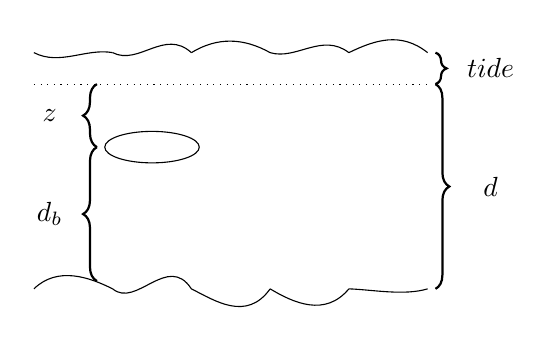
\begin{tikzpicture}
%Water surface
\draw (0,0) .. controls (0.33,-0.17) and (0.66,0.06) .. (1,0);
\draw (1,0) .. controls (1.33,-0.17) and (1.66,0.31) .. (2,0);
\draw (2,0) .. controls (2.33,0.2) and (2.66,0.19) .. (3,0);
\draw (3,0) .. controls (3.33,-0.1) and (3.66,0.26) .. (4,0);
\draw (4,0) .. controls (4.33,0.16) and (4.66,0.27) .. (5,0);

\draw[dotted] (0,-0.4) -- (5,-0.4);

%AUV
%\draw[rotate=25] (1,-1.7) ellipse (0.6 and 0.2);
\draw (1.5,-1.2) ellipse (0.6 and 0.2);

\draw (0,-3) .. controls (0.3,-2.71) and (0.7,-2.85) .. (1,-3);
\draw (1,-3) .. controls (1.3,-3.25) and (1.7,-2.54) .. (2,-3);
\draw (2,-3) .. controls (2.3,-3.15) and (2.7,-3.42) .. (3,-3);
\draw (3,-3) .. controls (3.3,-3.18) and (3.7,-3.36) .. (4,-3);
\draw (4,-3) .. controls (4.3,-3.01) and (4.7,-3.09) .. (5,-3);

%Curli braces
\draw [decorate, decoration={brace, amplitude=5pt, mirror}, thick] (5.1, -3)  -- (5.1, -0.4) 
 node[label, midway, xshift=7mm] {$d$};
\draw [decorate, decoration={brace, amplitude=4pt, mirror}, thick] (5.1, -0.4)  -- (5.1, 0) 
 node[label, midway, xshift=7mm] {$tide$};
 
\draw [decorate, decoration={brace, amplitude=5pt, mirror}, thick] (0.8, -0.4)  -- (0.8, -1.2) 
 node[label, midway, xshift=-6mm] {$z$};
\draw [decorate, decoration={brace, amplitude=5pt, mirror}, thick] (0.8, -1.2)  -- (0.8, -2.9) 
 node[label, midway, xshift=-6mm] {$d_b$};

\end{tikzpicture}
  \caption{Bottom distance diagram. Here $d_b$ is the distance from the bottom, $d$ is the depth from the bathymetry data, $tide$ is the tide level and $z$ is the vehicle height.}
  \label{bottom_distance_diagram}
\end{figure}

\par The \textbf{updateForwardDistance} method calculates the distance from the vehicle nose to a forward barrier, which can be ocean floor, water surface or a line obstacle such as a pier. To do this it calls on the \textit{forwardRange} method, which returns the forward distance between nose and barrier, adds a randomly generated value to simulate measurement error, trims this final value to fit in the range $\left[d_{min}, d_{max}\right]$ and dispatches the forward \textit{Distance} message. 

\par The \textbf{forwardRange} method returns the distance to a a barrier depending on the vehicles pitch angle $\theta$. When $\theta > 0$ the method calculates the distance from the nose to the water surface, provided the max sensor range can intercept it, by using the formula: $d_f = \left| \frac{z}{\sin \left( \theta \right)} \right|$, as seen in figure \ref{forward_distance_surface}.

\begin{figure}[h]
  \centering
  	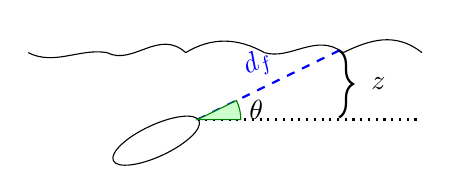
\begin{tikzpicture}
%Water surface
\draw (0,0) .. controls (0.33,-0.17) and (0.66,0.06) .. (1,0);
\draw (1,0) .. controls (1.33,-0.17) and (1.66,0.31) .. (2,0);
\draw (2,0) .. controls (2.33,0.2) and (2.66,0.19) .. (3,0);
\draw (3,0) .. controls (3.33,-0.1) and (3.66,0.26) .. (4,0);
\draw (4,0) .. controls (4.33,0.16) and (4.66,0.27) .. (5,0);

%AUV
\draw[rotate=25] (1,-1.7) ellipse (0.6 and 0.2);

%Aux
\draw[dashed, thick, blue] (2.15,-0.85) -- ++(26:2) node[midway, above, rotate=25]{$d_f$};
\draw[dotted, thick] (2.15,-0.85) -- (5,-0.85);
%Angles
\filldraw[fill=green!20,draw=green!50!black] (2.15,-0.85) -- ++(0.55,0) arc (0:26:0.55) node[midway, right] {$\theta$} -- cycle; 

%Curli braces
\path (2.15,-0.85)++(26:2) coordinate (water); 
\draw [decorate, decoration={brace, amplitude=5pt, mirror}, thick] (water)++(0,-0.85)  -- (water)
 node[label, midway, xshift=5mm] {$z$};

\end{tikzpicture}
  \caption{Forward distance to water surface diagram. Here $d_f$ is the distance to water surface, $\theta$ is pitch angle and $z$ is the vehicle height.}
  \label{forward_distance_surface}
\end{figure}

When $\theta < 0$  the method calculates the distance from the nose to the ocean floor. This can be done using two methods depending on the ``intersect\_method" flag. When the flag is disabled the method used, similar to the one described above, uses the formula: $d_f = \left| \frac{d_b}{\sin \left( \theta \right)} \right|$, as seen in figure \ref{forward_distance_floor_simple}.

\begin{figure}[h]
  \centering
  	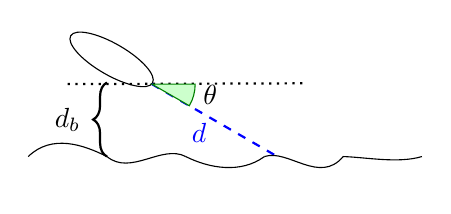
\begin{tikzpicture}

%AUV
\draw[rotate=-30] (1.8,-1) ellipse (0.6 and 0.2);

%Aux
\coordinate (F) at (1.57,-2.08);
\draw[dotted, thick] (0.5,-2.08) -- (3.5,-2.07);
\draw[dashed, thick, blue] (F) -- ++(-30:1.85) node[midway, below, xshift=-2mm, yshift=1mm] {$d$};
%Angles
\filldraw[fill=green!20,draw=green!50!black] (F) -- ++(0.55,0) arc (0:-30:0.55) node[midway, right] {$\theta$} -- cycle; 

%Ocean floor
\draw (0,-3) .. controls (0.3,-2.71) and (0.7,-2.85) .. (1,-3);
\draw (1,-3) .. controls (1.3,-3.25) and (1.7,-2.84) .. (2,-3);
\draw (2,-3) .. controls (2.3,-3.15) and (2.7,-3.22) .. (3,-3);
\draw (3,-3) .. controls (3.3,-2.90) and (3.7,-3.36) .. (4,-3);
\draw (4,-3) .. controls (4.3,-3.01) and (4.7,-3.09) .. (5,-3);

%Curli braces
\draw [decorate, decoration={brace, amplitude=5pt, mirror}, thick] (1,-2.06)  -- (1,-3)
 node[label, midway, xshift=-5mm] {$d_b$};

\end{tikzpicture}
  \caption{Forward distance to ocean floor diagram. Here $d_f$ is the distance to the ocean floor, $\theta$ is pitch angle and $d_b$ is the distance to bottom.}
  \label{forward_distance_floor_simple}
\end{figure}

When the flag is enabled the distance is computed by using a more complex algorithm, implemented in the \textbf{bottomIntersection} method. The algorithm computes the distance to bottom of a configurable number of points in front of the vehicle, spaced by an equal interval $\Delta x$. Then, these points are interpolated to create a rough outline of the ocean surface in front of the vehicle. The coordinates corresponding to the end of the echo sounder's lower beam $\left(x_{lb}, z_{lb}\right)$ are then computed using: $x_{lb} = d_{max} \cos\left(\theta - \alpha \right)$ and $z_{lb} = - d_{max} \sin\left(\theta - \alpha \right) + z$, where $d_{max}$ is the maximum sensor range and $\alpha$ is half of the sensor's width angle, as seen in figure \ref{forward_distance_floor_complex}. Then we check for an intersection between the lower beam and the rough floor profile (red point in figure \ref{complex_geometry}) and, if one is found, its distance from the forward sensor is calculated.

\begin{figure}[h]
    \centering
    %PROFILE
    \begin{subfigure}[b]{0.4\textwidth}
        \begin{tikzpicture}
%AUV
\draw[rotate=-30] (-0.6,0) ellipse (0.6 and 0.2);

%Bottom profile
\draw (0,-3) .. controls (0.3,-2.09) and (0.7,-2.69) .. (1,-3);
\draw (1,-3) .. controls (1.3,-2.64) and (1.7,-4.0) .. (2,-3);
\draw (2,-3) .. controls (2.3,-2.26) and (2.7,-3.11) .. (3,-3);
\draw (3,-3) .. controls (3.3,-3.92) and (3.7,-2.09) .. (4,-3);
\draw (4,-3) .. controls (4.3,-3.91) and (4.7,-3.66) .. (5,-3);

%Curli braces
\draw [decorate, decoration={brace, amplitude=5pt, mirror}, thick] (0.5, 1)  -- (0, 1) 
 node[label, xshift=2mm, yshift=5mm] {$\Delta x$};
\draw [decorate, decoration={brace, amplitude=5pt, mirror}, thick]  (5, -3.6) -- (5, 1) 
 node[label, rotate= -90, midway, yshift=5mm] {$depth$}; %xshift=2mm, yshift=5mm

%Dots and distance lines
\draw[dotted](0, 1) - - (0, -3);
\filldraw[black](0, 1) circle(1.5pt);
\filldraw[black](0, -3) circle(1.5pt);
\draw[dotted](0.5, 1) - - (0.5, -2.55);
\filldraw[black](0.5, 1) circle(1.5pt);
\filldraw[black](0.5, -2.55) circle(1.5pt);
\draw[dotted](1, 1) - - (1, -3);
\filldraw[black](1, 1) circle(1.5pt);
\filldraw[black](1, -3) circle(1.5pt);
\draw[dotted](1.5, 1) - - (1.5, -3.25);
\filldraw[black](1.5, 1) circle(1.5pt);
\filldraw[black](1.5, -3.25) circle(1.5pt);
\draw[dotted](2, 1) - - (2, -3);
\filldraw[black](2, 1) circle(1.5pt);
\filldraw[black](2, -3) circle(1.5pt);
\draw[dotted](2.5, 1) - - (2.5, -2.75);
\filldraw[black](2.5, 1) circle(1.5pt);
\filldraw[black](2.5, -2.75) circle(1.5pt);
\draw[dotted](3, 1) - - (3, -3);
\filldraw[black](3, 1) circle(1.5pt);
\filldraw[black](3, -3) circle(1.5pt);
\draw[dotted](3.5, 1) - - (3.5, -3);
\filldraw[black](3.5, 1) circle(1.5pt);
\filldraw[black](3.5, -3) circle(1.5pt);
\draw[dotted](4, 1) - - (4, -3);
\filldraw[black](4, 1) circle(1.5pt);
\filldraw[black](4, -3) circle(1.5pt);
\draw[dotted](4.5, 1) - - (4.5, -3.6);
\filldraw[black](4.5, 1) circle(1.5pt);
\filldraw[black](4.5, -3.6) circle(1.5pt);

\end{tikzpicture}
        \caption{Floor profiling diagram.}
        \label{complex_profile}
    \end{subfigure}
    ~\hfill%GEOMETRY
    \begin{subfigure}[b]{0.4\textwidth}
        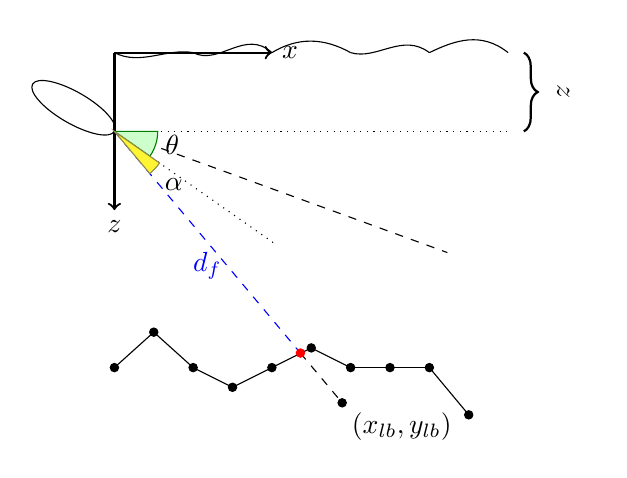
\begin{tikzpicture}
%AUV
\draw[rotate=-30] (-0.6,0) ellipse (0.6 and 0.2);

%Axis
\draw[thick,->] (0,1) -- (2,1) node[right] {$x$};
\draw[thick,->] (0,1) -- (0,-1) node[below] {$z$};

%Water surface
\draw (0,1) .. controls (0.33,-0.17+1) and (0.66,0.06+1) .. (1,1);
\draw (1,1) .. controls (1.33,-0.17+1) and (1.66,0.31+1) .. (2,1);
\draw (2,1) .. controls (2.33,0.20+1) and (2.66,0.19+1) .. (3,1);
\draw (3,1) .. controls (3.33,-0.1+1) and (3.66,0.26+1) .. (4,1);
\draw (4,1) .. controls (4.33,0.16+1) and (4.66,0.27+1) .. (5,1);

%Aux
\draw[dotted] (0,0) -- (5,0);

%Curli Braces
\draw [decorate, decoration={brace, amplitude=5pt, mirror}, thick]  (5.2, 0) -- (5.2, 1) 
 node[label, rotate= -90, midway, yshift=5mm] {$z$}; %xshift=2mm, yshift=5mm

%Bottom interpolation
\filldraw[black](0, -3) circle(1.5pt);
\draw[black](0, -3) -- (0.5, -2.55);
\filldraw[black](0.5, -2.55) circle(1.5pt);
\draw[black](0.5, -2.55) -- (1, -3);
\filldraw[black](1, -3) circle(1.5pt);
\draw[black](1, -3) -- (1.5, -3.25);
\filldraw[black](1.5, -3.25) circle(1.5pt);
\draw[black](1.5, -3.25) -- (2, -3);
\filldraw[black](2, -3) circle(1.5pt);
\draw[black](2, -3) -- (2.5, -2.75);
\filldraw[black](2.5, -2.75) circle(1.5pt);
\draw[black](2.5, -2.75) -- (3, -3);
\filldraw[black](3, -3) circle(1.5pt);
\draw[black](3, -3) -- (3.5, -3);
\filldraw[black](3.5, -3) circle(1.5pt);
\draw[black](3.5, -3) -- (4, -3);
\filldraw[black](4, -3) circle(1.5pt);
\draw[black](4, -3) -- (4.5, -3.6);
\filldraw[black](4.5, -3.6) circle(1.5pt);

%Beam limits
\draw[dashed] (0,0) -- (-20:4.5);
\draw[dotted] (0,0) -- (-35:2.5);
\draw[dashed, blue] (0,0) -- (-50:3.675) node[midway, below] {$d_f$};
\draw[dashed] (-50:3.675) -- (-50:4.5);
\filldraw[red](-50:3.675) circle(1.5pt);
\filldraw[black](-50:4.5) circle(1.5pt) node[below right] {$\left(x_{lb}, y_{lb}\right)$};
%Angles
\filldraw[fill=green!20,draw=green!50!black] (0,0) -- (0.55,0) arc (0:-35:0.55) node[midway, right] {$\theta$} -- cycle; 
\filldraw[fill=yellow!80,draw=yellow!50!black] (0,0) -- (-35:0.7) arc (-35:-50:0.7) node[midway, below right] {$\alpha$} -- cycle;

\end{tikzpicture}
        \caption{Algorithm geometry diagram.}
        \label{complex_geometry}
    \end{subfigure}
    \caption{Forward distance to ocean floor, complex method diagram. In figure \ref{complex_profile} $\Delta x$ is the forward step. In figure \ref{complex_geometry} $\theta$ is pitch angle, $\alpha$ is half of the sensor's width angle, $\left(x_{lb},y_{lb}\right)$ are the coordinates for the end of the echo sounder's lower beam and $d_f$ is the desired forward distance.}
    \label{forward_distance_floor_complex}
\end{figure}

If the ``simulate\_pier" flag is enabled, the \textit{forwardRange} method computes the distance to the virtual pier. The algorithm computes the coordinates corresponding to the maximum forward sensor range $\left(x_{fr}, y_{fr}\right)$, using: $x_{fr} = x + d_{max} \cos\left(\psi + \psi_{pb} \right)$ and $y_{fr} = y + d_{max} \sin\left(\psi + \psi_{pb} \right)$, where $\left(x, y\right)$ is the vehicle's position over ground (in the gps offset coordinates), $\psi$ is the vehicle's yaw and $\psi_{pb}$ is the angle of the scanner beam in pencil beam scanning, as seen in figure \ref{forward_distance_pier}. Then we check for an intersection between this forward beam and the virtual pier, simulated by the points $\left\{\left(x_a,y_a\right), \left(x_b,y_b\right)\right\}$. If it does the distance to the intersection point is calculated. Finally the minimum distance value between $d_{max}$, water surface/ocean floor and pier is returned as the forward distance.

\begin{figure}[h]
  \centering
  	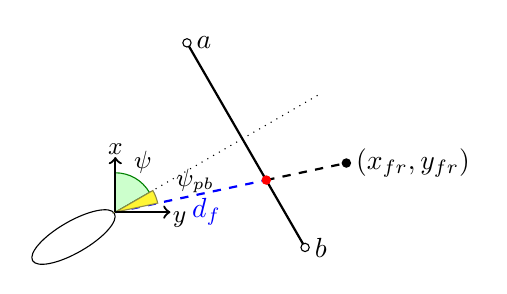
\begin{tikzpicture}

%AUV
\draw[rotate=30] (1.8,-1) ellipse (0.6 and 0.2);

%Pier
\path (3.5,2.5) coordinate (a);
\path (a)++(-60:3) coordinate (b);
\draw[thick] (a) -- (b);
\filldraw[fill=white, draw=black](a) circle(1.5pt) node[right]{$a$};
\filldraw[fill=white, draw=black](b) circle(1.5pt) node[right]{$b$};

%Aux
\path (2.59,0.35) coordinate (f);
\draw[dotted] (f) -- ++(30:3);
\draw[dashed, thick, blue] (f) -- ++(12:1.96) node[midway, below, xshift=2mm, yshift=1mm] {$d_f$};
\draw[dashed, thick] (f)++(12:1.96) -- ++(12:1.04);
%Angles
\filldraw[fill=green!20,draw=green!50!black] (f) -- ++(0,0.5) arc (90:30:0.5) node[midway, xshift=1mm, yshift=2mm] {\small $\psi$} -- cycle; 
\filldraw[fill=yellow!80,draw=yellow!50!black] (f) -- ++(30:0.55) arc (30:12:0.55) node[midway, xshift=5mm, yshift=2mm] {\small $\psi_{pb}$} -- cycle;

%Points
\filldraw[black](f)++(12:3) circle(1.5pt) node[right]{$\left(x_{fr},y_{fr}\right)$};
\filldraw[red](f)++(12:1.96) circle(1.5pt);

%Axis
\draw[thick,->] (f) -- ++(0.7,0) node[right, xshift=-1mm, yshift=-1mm] {\small $y$};
\draw[thick,->] (f) -- ++(0,0.7) node[above, yshift=-1mm] {\small $x$};

\end{tikzpicture}
  \caption{Forward distance to simulated pier diagram. Here $a$ and $b$ are the points delimiting the simulated pier, $d_f$ is the distance to the pier, $\psi$ is the yaw angle, $\psi_{pb}$ is the angle of the scanner beam and $\left(x_{fr}, y_{fr}\right)$ are the coordinates of the maximum forward sensor range.}
  \label{forward_distance_pier}
\end{figure}


\section{Leaks Task \href{https://www.lsts.pt/docs/dune/dune-2017.01.0-dmsmw/d2/d45/structSimulators_1_1Leaks_1_1Task.html}{\textsuperscript{*}}}

\par The simulator's Leaks task is responsible for simulating a leak detection inside the vehicle, in the same way a hardware leak sensor would. This is done by sending a manual \textit{LeakSimulation} message which triggers a report from leak sensor entities indicating a leak detection.

\par When the task is started names of the leak entities to simulate are taken from the configuration file. The \textbf{onEntityReservation} method then reserves the entity ids for the number of simulators specified, using the respective label names, and the entity pointers are saved in a stateful entity vector ``m\_leaks". These are initialized with normal state (``ESTA\_NORMAL").

\par The task consumes a \textcolor{red}{manually sent} \textit{LeakSimulation} message. This message contains a list of entities a desired state, ON or OFF. The method then assigns the desired state to all leak entities whose labels correspond to those of the received list, and calls on the \textbf{reportState} method for each one, dispatching an \textit{EntityState} message.

This message contains a list of entities it refers to and a field indicating if a leak simulation should be ON or OFF. In the case of an empty list the method simply assigns the received state to all entities in the ``m\_leaks" vector assigning the states ``ESTA\_NORMAL" or ``ESTA\_FAILURE", where failure indicates a leak. If a non-empty list is received the method assigns the received state to all corresponding entities and calls on the \textbf{reportState} method for each one, which dispatches an \textit{EntityState} message. In the case of an empty list the method simply assigns the desired state to all entities in the ``m\_leaks" vector.

\section{Gaussian Task \href{https://www.lsts.pt/docs/dune/dune-2017.01.0-dmsmw/d9/d36/structSimulators_1_1Gaussian_1_1Task.html}{\textsuperscript{*}}}

\par The simulator's Gaussian task is capable of simulating generalized quantities, such as temperature, sound speed, pressure, etc.. The quantities follow a 2D gaussian profile with a small random element. The simulated value can be dispatched via a generic IMC message, which can be configured to be of any message type that contains a ``value" field.

\par The \textbf{onUpdateParameters} method coverts all angular quantities from degrees to radians.  It also initializes the generic message pointer, that will dispatch the final value, according to the configured message type: \textit{Temperature}, \textit{SoundSpeed}, \textit{Pressure}, etc.

\par The task consumes \textit{SimulatedState} messages that are used to obtain the vehicle's position.

\par In order to simulate the values the periodic task implements a gaussian profile in the form: $value = \Omega +\left(\mu - \Omega\right) \exp\left(-\frac{\left(x - x_0\right)^2+\left(y - y_0\right)^2 }{2\sigma^2}\right)$, where $\left(x_0, y_0\right)$ is the peak position, in WGS84 coordinates, $\sigma^2$ is the standard deviation, $\mu$ is the maximum peak value and $\Omega$ is the minimum value when far from the peak. These profile parameters can be set in the configuration file. The variables $\left(x, y\right)$ are the vehicle's coordinates obtained from the received \textit{SimulatedState}. The task first calculates the vehicle position, by adding the position offsets to the GPS origin, and then calculates its displacement from the peak's position $\left(x-x_0, y-y_0 \right)$. A small random value is then added to simulate perturbations. Finally the value is assigned to the message and dispatched. It is also possible to activate invalid readings when at the surface via the ``invalid" flag. In this case, if a vehicle is above a configurable threshold a value of -1 is dispatched, indicating an invalid reading.

\section{CTD Task \href{https://www.lsts.pt/docs/dune/dune-2017.01.0-dmsmw/dd/df2/structSimulators_1_1CTD_1_1Task.html}{\textsuperscript{*}}}

\par The simulator's \textbf{C}onductivity \textbf{T}emperature and \textbf{D}epth task is responsible for simulating environmental parameters such as: temperature, salinity, depth, pressure, conductivity and sound speed, by sending \textit{Temperature}, \textit{Salinity}, \textit{Depth}, \textit{Pressure}, \textit{Conductivity} and \textit{SoundSpeed} messages, respectively. To this end it uses collected temperature and salinity data to simulate those quantities directly and performs calculations to simulate the remaining parameters. The task is also capable of time dependent simulation using multiple data files for different time points.

\par The \textbf{onResourceInitialization} method initializes two \textbf{DataParameters} objects, to hold the temperature and salinity data. The constructor calls on the \textbf{filltree} member method to parse the configurable data files, currently in \path{etc/simulation/}. Each file contains a reference origin latitude and longitude, in WGS84 coordinates, and a series of data points in the form ``$x\ y\ z\ d$" where $x$, $y$ and $z$ are the offsets from the origin, in $m$, and $d$ is the data value at that point and analogous to the Environment task the data is used to populate an octree structure. However, here, the process is repeated to parse the files with data at different time points. Finally, after parsing the data, the method deactivates the task to be reactivated when a \textit{SimulatedState} message is received.

\par The \textbf{onResourceAcquisition} method initializes a Random::Generator object, later used to simulate measurement error.

\par The task consumes an initial \textit{GpsFix} message, of the manual input type, from the GPS simulator, containing the reference origin coordinates used in navigation. The method then sets the displacement between the gps and data reference origins in each \textbf{DataParameter} object, allowing us to easily convert our coordinates between reference frames.

\par The \textit{SimulatedState} consume method saves the \textit{SimulatedState} message sent by the VSIM task, which will be used to obtain the vehicles position. The method also activates the task, if not active, and initializes the timer used to obtain the relative time for the time dependent simulation.

\par The periodic task is responsible for dispatching all parameter messages. The temperature and salinity values are obtained by calling the \textbf{valueAt} member function of \textbf{DataParameters}. The depth value is simply obtained from the \textit{SimulatedState} $z$ field. The pressure, in bar, is computed using the formula: $p = z \cdot \rho \cdot g + p_0$, where $z$ is the vehicle depth, $\rho$ is the water density, $g$ is gravitational acceleration and $p_0$ is the pressure at sea level. The water conductivity and sound speed are computed using the respective algorithms found in \cite{UNESCO}, using the temperature, salinity and pressure parameters as inputs. A randomly generated value is then added to these quantities to simulate measurement error and the messages are dispatched.

\par The \textbf{valueAt} method returns the parameter value at the specified time and location. In case the specified time is outside the time window of the data set the returned value is obtained from the data set with the closest time, using the \textbf{interpolateSpaceAt} method. When the time falls within the time window of the data set a linear interpolation ($d = m \cdot t + b$) is made to determine the value. The coefficient $m$ is obtained using $m = \frac{d_{after} - d_{before}}{t_{after} - t_{before}}$, where $t_{after}$ is the time of the closest future data set and $d_{after}$ is the corresponding parameter value, $t_{before}$ and $d_{before}$ are analogous for the closest past data set. The coefficient $b$ is obtained using $b = d_{before} - m \cdot t_{before}$. The parameter value is then returned for the specified time using $d_{specified} = m \cdot t_{specified} + b$.

\par The \textbf{interpolateSpaceAt} method performs a spatial interpolation using inverse distance weighting, at the specified location on a specified data set (time). Here we search the octree for all points in a given interpolation radius around the specified location and return an average value weighted by distance.

\bibliographystyle{plain}
\bibliography{References}

\end{document}
